                                               %%%%%%%%%%%%%%%%%%%%%%%%%%%%%%%%%%%%%%%%%%%%%%%%%%%%%%%%%%%%%%%%%%%%%%%%%%%%%%%
%%% SWEAVE
       % Ihaka, R. (2009). Customizing Sweave 
%%%%%%%%%%%%%%%%%%%%%%%%%%%%%%%%%%%%%%%%%%%%%%%%%%%%%%%%%%%%%%%%%%%%%%%%%%%%%%%
%%% CUSTOMIZING SWEAVE 
%%% from: Ihaka, R. (2009). Customizing Sweave to Produce Better Looking LATEX Output
\DefineVerbatimEnvironment{Sinput}{Verbatim}{fontsize=\footnotesize, formatcom=\color{codecolor}, xleftmargin=2em}
\DefineVerbatimEnvironment{Soutput}{Verbatim}{fontsize=\footnotesize, xleftmargin=2em, formatcom=\color{codecolor}} 
\DefineVerbatimEnvironment{Scode}{Verbatim}{fontsize=\footnotesize, xleftmargin=2em, formatcom=\color{codecolor}}

\renewenvironment{Schunk}{\vspace{10pt}}{\vspace{8pt}}   
%%%%%%%%%%%%%%%%%%%%%%%%%%%%%%%%%%%%%%%%%%%%%%%%%%%%%%%%%%%%%%%%%%%%%%%%%%%%%%%
%%%%%%%%%%%%%%%%%%%%%%%%%%%%%%%%%%%%%%%%%%%%%%%%%%%%%%%%%%%%%%%%%%%%%%%%%%%%%%%

\section{Stichprobenverteilung des Mittelwerts}

\begin{Schunk}
\begin{Sinput}
> mu <- 100
> s <- 10
> pop <- rnorm(1e3, mu, s)
> hist(pop, breaks=40, col="grey")
\end{Sinput}
\end{Schunk}
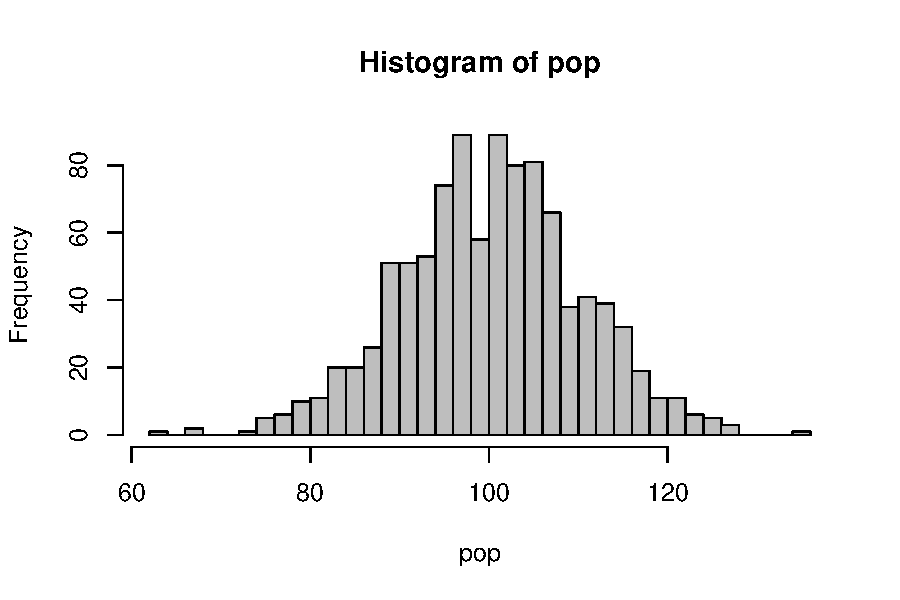
\includegraphics{sim_mean_dist-002}


\begin{Schunk}
\begin{Sinput}
> sample_means <- function(pop, n, nrep=1000){
   res <- rep(NA, nrep)
   for (i in 1:nrep)
     res[i] <- mean(sample(pop, n))  
   res
 }
\end{Sinput}
\end{Schunk}

\begin{Schunk}
\begin{Sinput}
> ns <- seq(10, 200, 40)
> l <- list()
> for (i in seq_along(ns)){
   means <- sample_means(pop, ns[i])
   l[[i]] <- data.frame(n=ns[i], means)  
 }       
> x <- do.call(rbind, l)
\end{Sinput}
\end{Schunk}

\begin{Schunk}
\begin{Sinput}
> library(ggplot2)
> ggplot(x, aes(x=means)) + geom_histogram(binwidth=.2) +
   facet_grid(. ~ n)
\end{Sinput}
\end{Schunk}
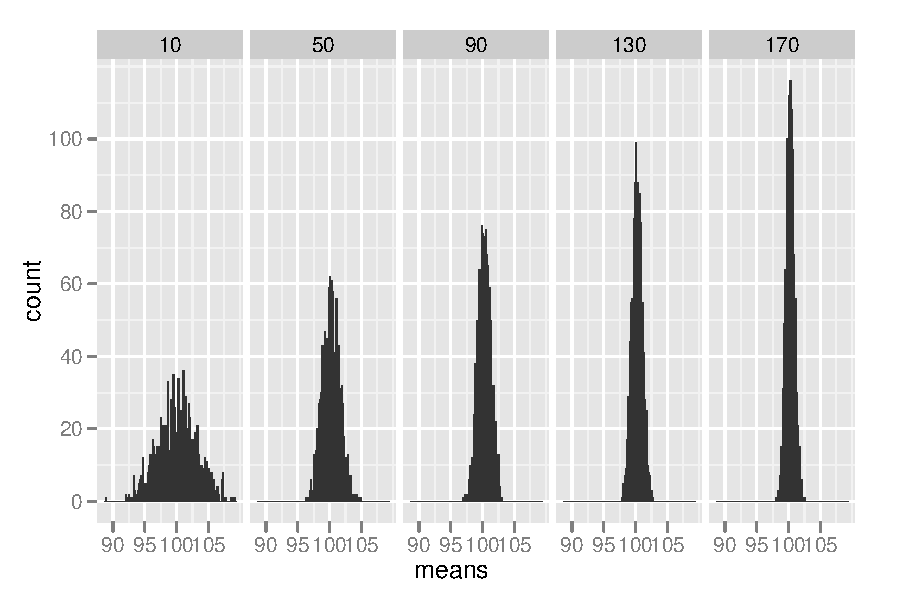
\includegraphics{sim_mean_dist-005}










